\section{Model}

In this section, we present the detailed design and architectural innovations of Qwen-Image-VAE-2.0. 



\subsection{Design Principle: High Compression VAE with Large Channel}

To optimize the training efficiency of downstream DiTs, we prioritize a higher spatial compression ratio. Given an input image $I \in \mathbb{R}^{H \times W \times 3}$, the VAE maps it to a latent representation $z \in \mathbb{R}^{\frac{H}{f} \times \frac{W}{f} \times C}$, where $f$ denotes the spatial compression ratio and $C$ represents the channel dimension. 
This results in a sequence length of $L = HW/f^2$ for the DiT. Since DiT's computational complexity scales quadratically with sequence length~\citep{attention}, the computation overhead of $\mathcal{O}(L^2)=\mathcal{O}(H^2W^2/{f^4})$ presents a significant bottleneck in high-resolution image generation.

To alleviate this, we move beyond the conventional $f8$ paradigm~\citep{rombach2022high, flux2024, wan2025wan}, adopting higher compression ratios of $f16$ and $f32$ to significantly reduce DiT training costs. While high spatial compression ratio $f$ promises training efficiency, it inevitably constrains the information capacity of the latent space, often resulting in the loss of fine-grained structural detail. To mitigate this, we rely on the principle that reconstruction fidelity is largely governed by the total information bottleneck $N(z)={CHW}/{f^2}$~\citep{dcae}. By increasing the channel dimension $C$, we compensate for the spatial information loss incurred by high compression ratio $f$. Notably, channel expansion does not compromise DiT training efficiency: during training, the DiT first projects latents into a fixed hidden dimension via a linear layer, ensuring that the computational complexity remains nearly invariant to channel dimension.

\subsection{Model Architecture}
\begin{figure}[htbp]
    \centering
    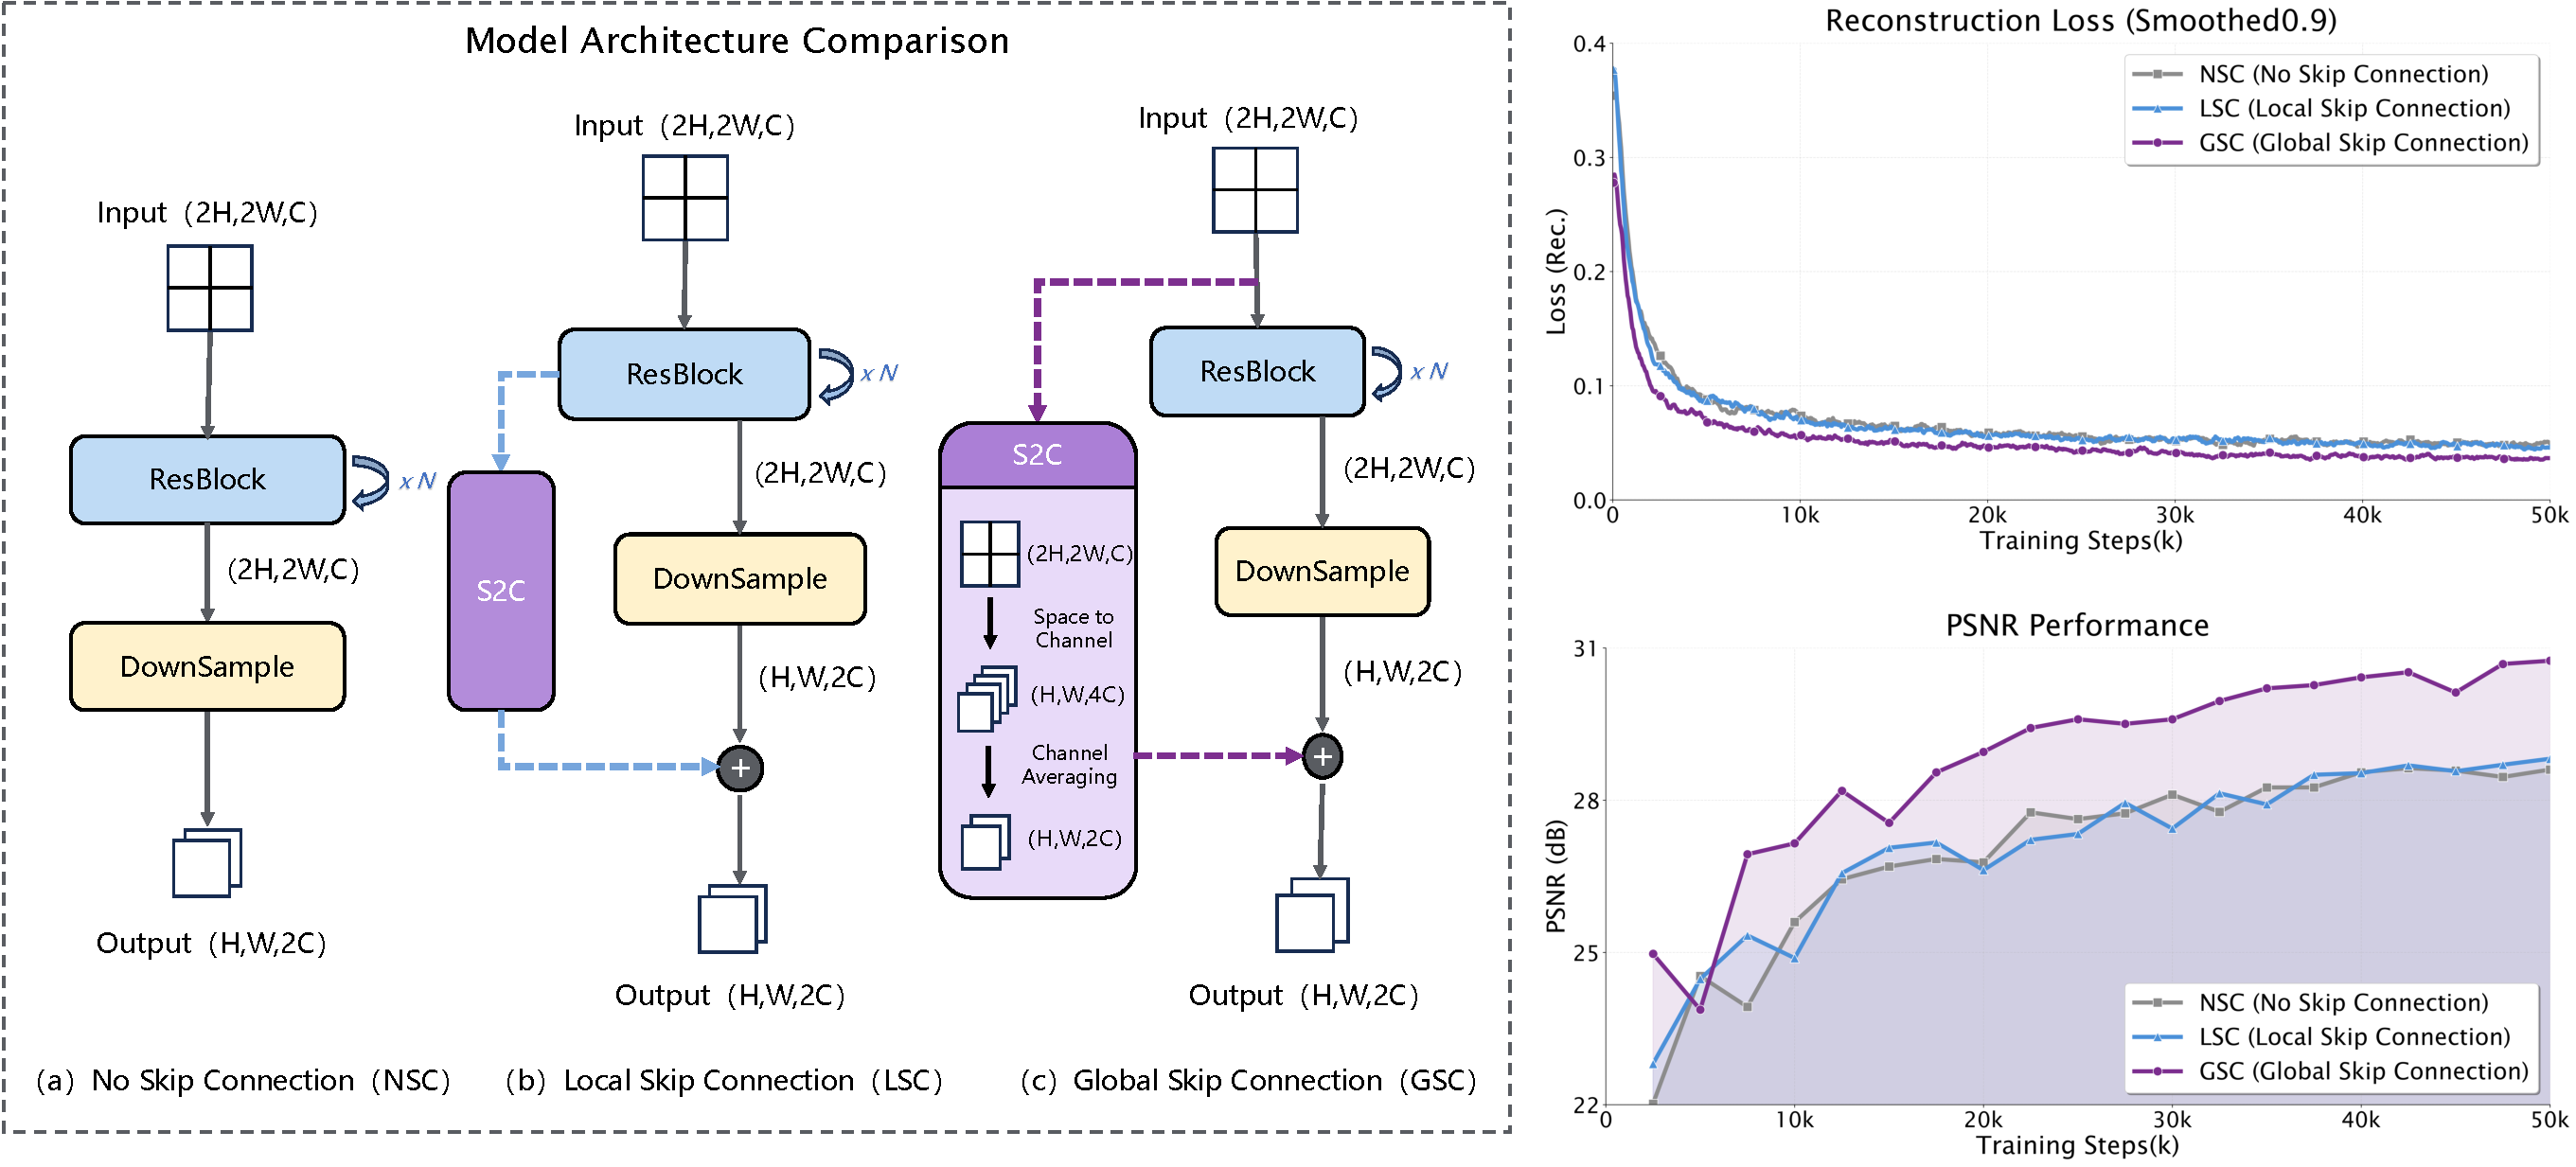
\includegraphics[width=1.0\linewidth]{pics/vae_report_arch.pdf}
    \caption{Comparison of No Skip Connection (NSC), Local Skip Connection (LSC), and Global Skip Connection (GSC) on model architecture, reconstruction loss and PSNR performance. S2C is the abbreviation of Space to Channel module. The experiments are conducted on $f16c64$ model training from scratch.}
    \label{fig:vae_arch}
\end{figure}


\paragraph{Global Skip Connection (GSC).}
A primary challenge in high-compression VAEs is the preservation of fine-grained detail during the aggressive downsampling process. The encoder, particularly its non-parametric downsampling layers, often struggles to retain high-frequency information from the original image, leading to optimization difficulties and blurry reconstructions~\citep{dcae}. To alleviate this information loss, we introduce the Global Skip Connection (GSC).

The GSC establishes a direct residual path that bypasses the initial downsampling stage, feeding pixel-level information directly into the deeper latent space. As illustrated in Figure~\ref{fig:vae_arch}, we implement this by employing a space-to-channel operation followed by reshaping, which effectively "folds" spatial information from the input image into the channel dimension.

To validate the efficacy of this design, we conducted an ablation study comparing three configurations: No Skip Connection (NSC), Local Skip Connection (LSC), and Global Skip Connection (GSC). Experiments on an f16c64 model trained from scratch demonstrate that the GSC significantly accelerates convergence by providing the network with high-frequency signal from the input. Based on these findings, we integrate the GSC across the entire Qwen-Image-VAE-2.0 series.



\paragraph{Attention-Free Backbone.} 
For an input of sequence length $N$, the computational complexity of self-attention is $\mathcal{O}(N^2)$, whereas that of convolution with a kernel size $k$ is $\mathcal{O}(N \cdot k^2)$. This quadratic scaling with pixels creates a significant throughput bottleneck for high-resolution image processing. Moreover, the activation memory required for self-attention also scales as $\mathcal{O}(N^2)$, imposing a severe memory constraint during training. In addition, we observed no significant performance degradation when removing attention modules. Consequently, we adopt an attention-free backbone for the entire Qwen-Image-VAE-2.0 series to ensure both training efficiency and scalability.

\paragraph{Encoder-Decoder Asymmetry.} 
We adopt an asymmetric architecture to balance encoding speed with reconstruction quality. By employing a lightweight encoder, we streamline the latent extraction process, effectively reducing training latency for the downstream DiT. Meanwhile, the heavyweight decoder guarantees high-fidelity reconstruction and the preservation of intricate image detail.

\subsection{Model Configurations}

The detailed configurations of the Qwen-Image-VAE-2.0 series are summarized in Table~\ref{tab:vae_configs}.

\begin{table}[htbp]
\centering
\caption{Configurations of Qwen-Image-VAE-2.0 suite. $d_{enc}$ and $d_{dec}$ denote the first projected hidden dimensions of the encoder and decoder. $n_{\text{layer}}$ denotes the number of layers.}
\label{tab:vae_configs}
\begin{tabular}{lccccccc}
\toprule
\textbf{Model} & $f$ & $C$ & $d_{enc}$ & $d_{dec}$ & $n_{\text{layer}}$ & \textbf{Residual} & \textbf{\#Params (Enc/Dec)} \\ \midrule
Qwen-Image-VAE-2.0-f16c64  & 16 & 64  & 96 & 144 & 5 & GSC & 76M / 248M \\
Qwen-Image-VAE-2.0-f16c128  & 16 & 128  & 96 & 144 & 5 & GSC & 76M / 248M \\
Qwen-Image-VAE-2.0-f32c128 & 32 & 128 & 96 & 144 & 6 & GSC & 77M / 250M \\
Qwen-Image-VAE-2.0-f32c192 & 32 & 192 & 96 & 144 & 6 & GSC & 78M / 250M \\ \bottomrule
\end{tabular}
\end{table}
